\documentclass{article}
\usepackage{blindtext}
\usepackage[a4paper, total={18cm, 25cm}]{geometry}

% METH !!!!
\usepackage{amsmath}
\usepackage{amsthm}
\usepackage{amssymb}

\theoremstyle{definition}
\newtheorem{example}{Cv}[section]

% ----
\usepackage{tabularx}
\usepackage{mathtools}
\usepackage{booktabs}
\usepackage[czech]{babel}
\usepackage[useregional=numeric]{datetime2}
\usepackage{graphicx}
\usepackage{paralist}
\usepackage{pict2e}
\usepackage[dvipsnames]{xcolor}
\usepackage{setspace}

\DeclareRobustCommand{\slashcirc}{{\mathpalette\doslashcirc\relax}}

\makeatletter
\newcommand\doslashcirc[2]{%
  \sbox\z@{$#1\m@th\circ$}%
  \setlength\unitlength{\wd\z@}
  \begin{picture}(1,1)
  \roundcap
  \put(0,0){\box\z@}
  \put(0,0){\line(1,1){1}}
  \end{picture}%
}
\makeatother

\newcommand{\diameter}{$\slashcirc$ }

\newcommand{\TODO}[1]{
	\begin{large}
		\berry{
			(\textbf{TODO:}#1)
		}
	\end{large}
}

\def\doubleunderline#1{\underline{\underline{#1}}}

\newcommand{\red}[1]{\textcolor{Red}{#1}}
\newcommand{\blue}[1]{\textcolor{Blue}{#1}}
\newcommand{\green}[1]{\textcolor{Green}{#1}}
\newcommand{\brown}[1]{\textcolor{Brown}{#1}}
\newcommand{\yellow}[1]{\textcolor{Yellow}{#1}}
\newcommand{\magenta}[1]{\textcolor{Magenta}{#1}}
\newcommand{\lime}[1]{\textcolor{LimeGreen}{#1}}
\newcommand{\violet}[1]{\textcolor{Violet}{#1}}
\newcommand{\orange}[1]{\textcolor{Orange}{#1}}
\newcommand{\purple}[1]{\textcolor{Purple}{#1}}
\newcommand{\brick}[1]{\textcolor{BrickRed}{#1}}
\newcommand{\berry}[1]{\textcolor{WildStrawberry}{#1}}

% page command for new page easy use
\newcommand\page{\newpage}
% new paragraph without bold text
\newcommand{\para}[1]{
	\paragraph{\normalfont{#1}}
}

\newcommand{\bitem}[1]{\item \textbf{#1}} %bold item command
\newcommand{\mitem}[1]{\item \textbf{\large{#1}}} %main item command (large bold item)
\newcommand{\dtitem}[1]{\item[•] #1} %dot item
\newcommand{\dsitem}[1]{\item[-] #1} %dash item
\newcommand{\litem}[1]{\item \begin{large}
#1
\end{large}} %large item

% command for table of content but with new page command and no page numbering
\newcommand{\content}{\tableofcontents
    \thispagestyle{empty}
    \page}

% Section numbering to arabic
\renewcommand*\thesection{\arabic{section}}
\renewenvironment{itemize}[1]{\begin{compactitem}#1}{\end{compactitem}}
\renewenvironment{enumerate}[1]{\begin{compactenum}#1}{\end{compactenum}}
\renewenvironment{description}[0]{\begin{compactdesc}}{\end{compactdesc}}
\DeclarePairedDelimiter\abs{\lvert}{\rvert}
\newcommand{\frontpage}[2]{
\begin{center}
       \vspace{1cm}
       \begin{center}
       		\begin{small}
               Vyšší odborná škola ekonomická, sociální a zdravotnická, \break
		Obchodní akademie, Střední pedagogická škola a Střední zdravotnická škola, 
						Most, příspěvková organizace 
       		\end{small}
       \end{center}
		\vspace{\fill}
        \begin{center}
        		\begin{Huge}
        			\textbf{Seminární práce}
        		\end{Huge}
        	\end{center}
        	\begin{center}
        		\begin{Large}
        			\textbf{Sociální podnikání}
        		\end{Large}
        \end{center}
        %\vspace{16cm}
        \vspace{\fill}
        \begin{normalsize}
        		\begin{tabular}{p{0cm} p{1.5cm} p{10cm}}
        		& \textbf{Jméno:} & Martin Kopecký   \\
        		& \textbf{Třída:} & 1.R    \\
       	 	& \textbf{Obor:}  & Firemní ekonomika \\
        		& \textbf{Datum:} & \Today
        		\end{tabular}
        \end{normalsize}
    \end{center}
    \thispagestyle{empty}
    \page
}



\graphicspath{{../images/}}

\begin{document}

\section*{Matematika 1 teorie}
\subsection{\textbf{Opakování}}
\subsubsection{Značení}
* $\exists$ - existuje alespoň jedno \\
* $\forall$ - pro každý platí \\
* $N$ - přirozená čísla \\
* $Z$ - celá čísla \\
* $Q$ - racionální čísla ( zlomky $\rightarrow$ $\frac{1}{2}$...) \\
* $R$ - iracionální čísla ($\pi$,...) 
\subsubsection{\textbf{Zápis}}
\begin{tabular}{c || c}
    1) $\exists x \in N \forall y \in Z,x^2=y$ &
    2) $\forall x\in N \exists y \in Z, x^2=y$ \\
\end{tabular}
\subsubsection*{\textbf{Reálné funkce}}
\begin{description}
    \item \textbf{Elementární funkce} vzniká ze základních elementárních funkcí za pomocí 5 operací
    \item \textbf{$+$ , $-$, $*$, $/$, skládání}
    \item  konstantní funkce, mocniná funkce, exponenciální funkce
\end{description}

\subsection*{skládání}
\begin{tabular}{p{7.5cm} p{7.5cm}}
    \textbf{základní funkce} & \textbf{základní funkce} \\
    $y=\sin{x^2}$ & $y=\sin^2{x}$ \\
    \hline
    $f(x)=x^2$ & $f(x)=\sin{x}$  \\
    $g(y) = \sin{y}$ & $g(y) = y^2 $  \\
    $g(y)= \sin{f(x)} \Rightarrow y = \sin{x^2}$ & 
    $g(y)= f(x)^2 \Rightarrow y = \sin^2{x}$ \\
\end{tabular}
\\
\subsection*{Neelementární funkce}
Absolutní hodnota \\
\(
    \abs{x} = x ; x > 0 \\
    \abs{x} = 0 ; x = 0 \\
    \abs{x} = -x ; x < 0
\)
    \subsection*{Elementární funkce}
\begin{tabular}{p{6cm} p{6cm} p{6cm}}
    Konstantní funkce & Exponenciální funkce & Mocniná funkce \\
    $y = a$ & $y = a^x$ & $y = x^a$ \\
    $D_y=R$ & $D_y = R$ & $D_y = R$ \\
    $H_y = \{a\}$ & $H_y = (0;+\infty)$ & $H_y = (0;+\infty)$ \\ \\
    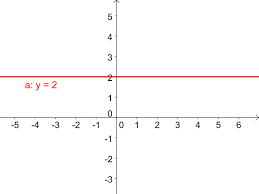
\includegraphics[scale=.5]{konst.png}&
    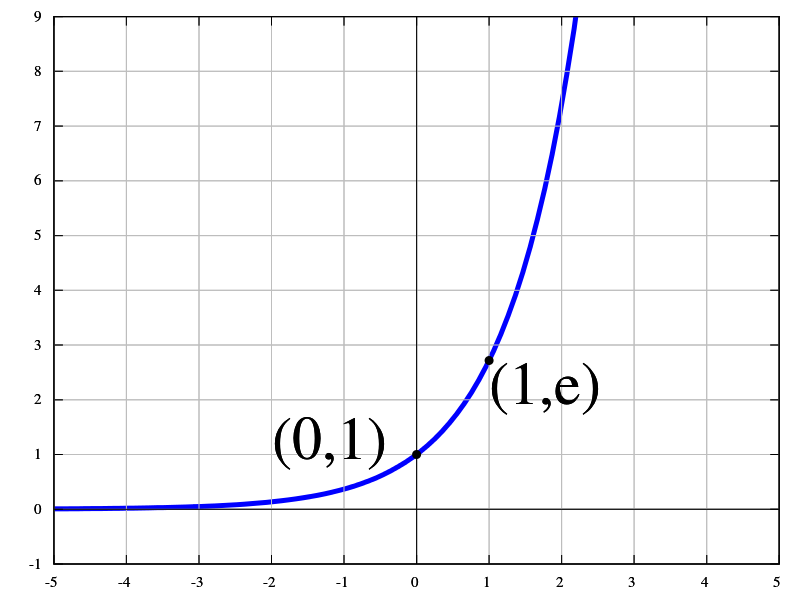
\includegraphics[scale=.2]{exp.png}&
    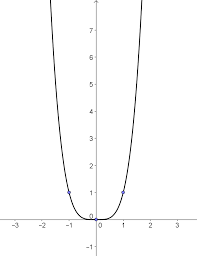
\includegraphics[scale=.5]{mocnina.png} \\

\end{tabular}

Goniometrocké fuknce
($\sin{},\cos{},\tan{}, \coth{}$)
 
\begin{center}
    \begin{tabular}{p{5cm} p{5cm}}
        \(\tan{x}=\frac{\sin{x}}{\cos{x}} \)&
        \(\coth{x}=\frac{\cos{x}}{\sin{x}} \) \\
    \end{tabular}
\end{center}
\page
\subsection*{10.10.2022}
\subsubsection*{Posloupnost a její limita}

\textbf{Omezenost}
\\\\
\begin{math}
    F N \rightarrow R
    \\ x_n = \frac{2n + 1}{3n}
    \\ 1 \rightarrow x_1 = 1
    \\ 2 \rightarrow x_2 = \frac{5}{6}
    \\\vdots
    \\ x_{10} = \frac{21}{30}
\end{math}
\\\\
$x_n$ je shora omezená  $<=>$ $\exists k \in R \forall n \in N , x_n \leqslant k$

\begin{gather*}
    k = 2
    \\ \frac{2n+1}{3n} \leq  2
    \\ 2n+1 \leq 6n
    \\ 1 \leq 4n
\end{gather*}

\textbf{Posloupnost konvergentní}
\begin{description}
    \dtitem{vlastní limita}   
    $ y_n = \frac{1}{n} \rightarrow 0 \\ \lim(y_n) = 0$
\end{description}

\begin{enumerate}
    \item $\frac{\infty}{\infty}$
    \begin{gather}
        \lim{\frac{3n-8}{56+2n}} = 
         \lim{\frac{\frac{3n}{2} - \frac{8}{n}}{\frac{56}{n}+\frac{2n}{n}}}
         \\
         \lim_{n\rightarrow\infty}{\frac{3n^2-8}{56+2n}} = \left[\frac{\infty}{\infty}\right] =
          \lim{\frac{\frac{3n^2}{n}-\frac{8}{n}}{\frac{56}{n}+\frac{2n}{n}}} =
          \lim{\frac{3n- \frac{8}{n}}{\frac{56}{n} + 2}} = \left[ \frac{\infty}{2}\right] = \doubleunderline{\infty}
        \\
        \lim{\frac{n!}{10^n}} \cong 0
        \\x_1 = 0.1
        \\x_2 = 0.02
        \\x_3 = 0.006
    \end{gather}
\end{enumerate}
\begin{align}
    \lim{(\sqrt{n^2+100}-n)}
\end{align}
\end{document}